\documentclass[letterpaper, 11pt]{article}
\usepackage[utf8]{inputenc}
\usepackage[letterpaper, portrait, margin=1in]{geometry}
\usepackage{pgfplots}
\pgfplotsset{width=10cm,compat=1.9}
\usepackage{hyperref}
\usepackage{textcomp}
\usepackage{siunitx}
\usepackage{amsmath}
\usepackage{cancel}
\usepackage{tikz}
\usepackage{everysel}
\usepackage{ragged2e}
\usepackage{mathdots}
\usepackage{yhmath}
\usepackage{color}
\usepackage{array}
\usepackage{multirow}
\usepackage{amssymb}
\usepackage{gensymb}
\usepackage{tabularx}
\usepackage{booktabs}
\usepackage{listings}
\usepackage{xcolor}
\usetikzlibrary{fadings}
\usetikzlibrary{patterns}
\usetikzlibrary{shadows.blur}
\hypersetup{
    colorlinks=true,
    linkcolor=black,
    filecolor=black,      
    urlcolor=blue,
}

\definecolor{codegreen}{rgb}{0,0.6,0}
\definecolor{codegray}{rgb}{0.5,0.5,0.5}
\definecolor{codepurple}{rgb}{0.58,0,0.82}
\definecolor{backcolour}{rgb}{0.95,0.95,0.92}

\lstdefinestyle{mystyle}{
    backgroundcolor=\color{backcolour},   
    commentstyle=\color{codegreen},
    keywordstyle=\color{magenta},
    numberstyle=\tiny\color{codegray},
    stringstyle=\color{codepurple},
    basicstyle=\ttfamily\footnotesize,
    breakatwhitespace=false,         
    breaklines=true,                 
    captionpos=b,                    
    keepspaces=true,                 
    numbers=left,                    
    numbersep=5pt,                  
    showspaces=false,                
    showstringspaces=false,
    showtabs=false,                  
    tabsize=2
}

\lstset{style=mystyle}

\title{COMSC-200 \\ Lab 1}
\author{Ryan Jacoby}
\date{6 September 2020}
\begin{document}

\maketitle

\section{Employee}
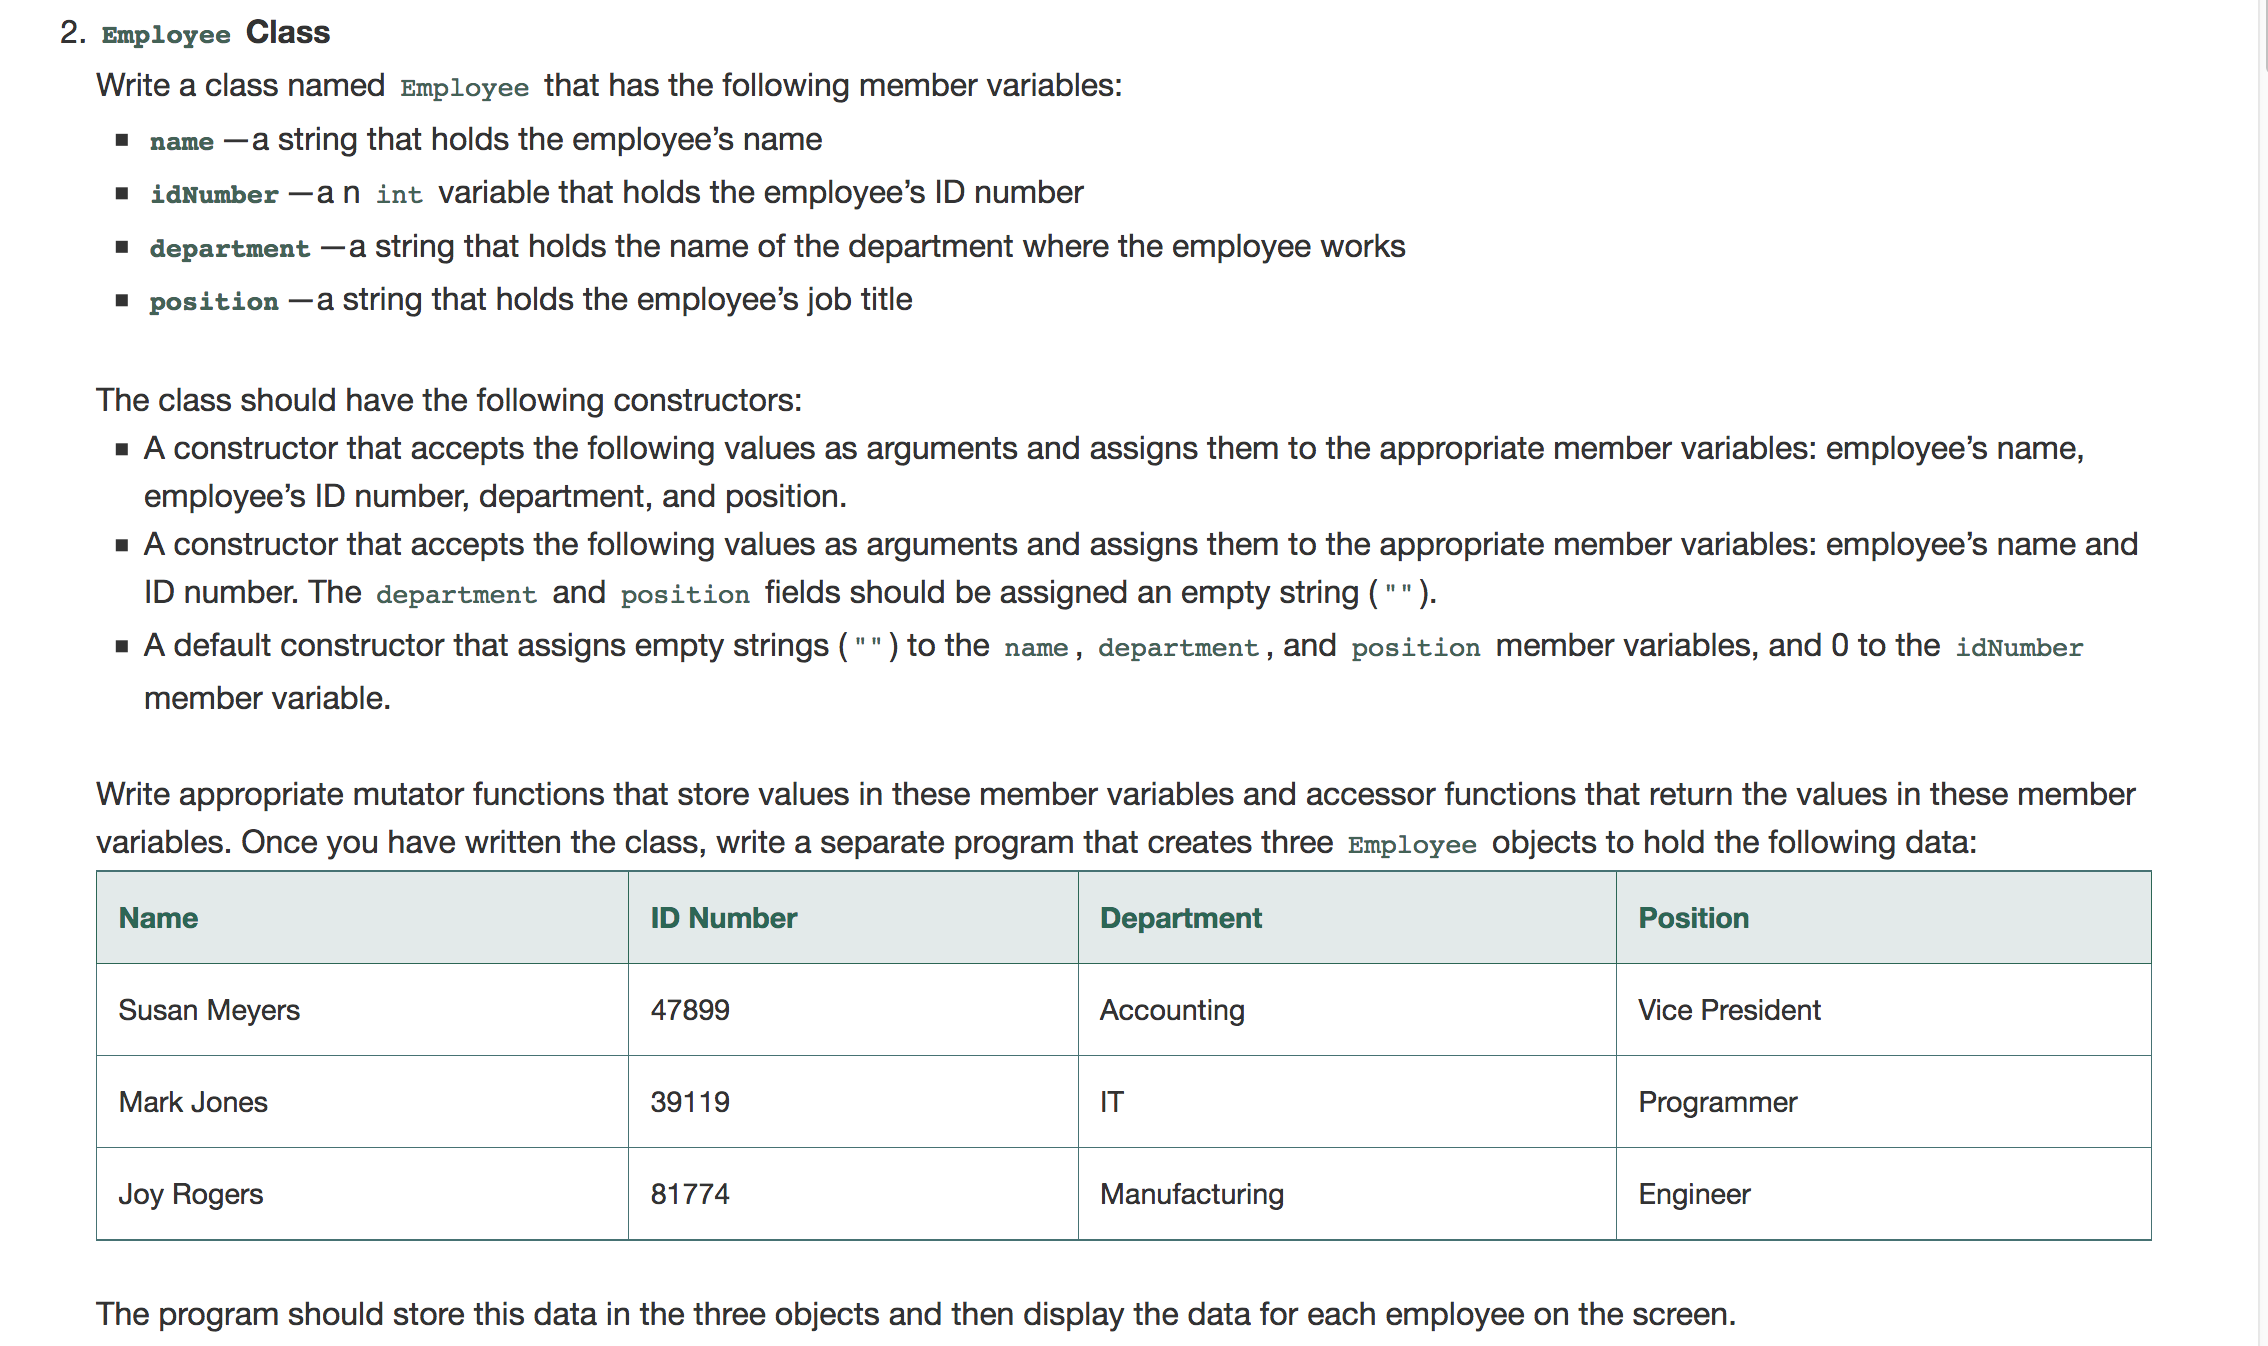
\includegraphics[scale=0.35]{employee.png} 

\begin{lstlisting}[language=C++, caption=main.cpp]
// Ryan Jacoby

#include<iostream>

#include"Employee.h"

using namespace std;

int main() {
    Employee employees[] = {Employee("Susan Meyers", 47899, "Accounting", "Vice President"),
                            Employee("Mark Jones", 39119, "IT\t", "Programmer"),
                            Employee("Joy Rodgers", 81774, "Manufacturing", "Engineer")};


    cout << "Name\t\tID Number\tDepartment\tPosition\n";
    for(int i = 0; i < 3; i++) 
        cout << employees[i].getName() << '\t' << employees[i].getIdNumber() << "\t\t" << employees[i].getDepartment() << '\t' << employees[i].getPosition() << '\n';

    return 0;
}    
\end{lstlisting}

\begin{lstlisting}[language=C++, caption=Employee.h]
// Ryan Jacoby

#ifndef Employee_h
#define Employee_h

using namespace std;

class Employee {
private:
    string name;
    int idNumber;
    string department;
    string position;
public:
    Employee();
    Employee(string name, int idNumber);
    Employee(string name, int idNumber, string department, string position);

    string getName() { return this->name; }
    int getIdNumber() { return this->idNumber; }
    string getDepartment() { return this->department; }
    string getPosition() { return this->position; }

    void setName(string name) { this->name = name; }
    void setIdNumber(int idNumber) { this-> idNumber = idNumber; }
    void setDepartment(string department) { this->department = department; }
    void setPosition( string position ) { this->position = position; }
};

#endif
\end{lstlisting}

\begin{lstlisting}[language=C++, caption=EmployeeImp.cpp]
// Ryan Jacoby

#include<string>

#include"Employee.h"

using namespace std;

Employee::Employee() {
    this->name = "";
    this->idNumber = 0;
    this->department = "";
    this->position = "";
}

Employee::Employee(string name, int idNumber) {
    this->name = name;
    this->idNumber = idNumber;
    this->department = "";
    this->position = "";
}

Employee::Employee(string name, int idNumber, string department, string position) {
    this->name = name;
    this->idNumber = idNumber;
    this->department = department;
    this->position = position;
}
\end{lstlisting}

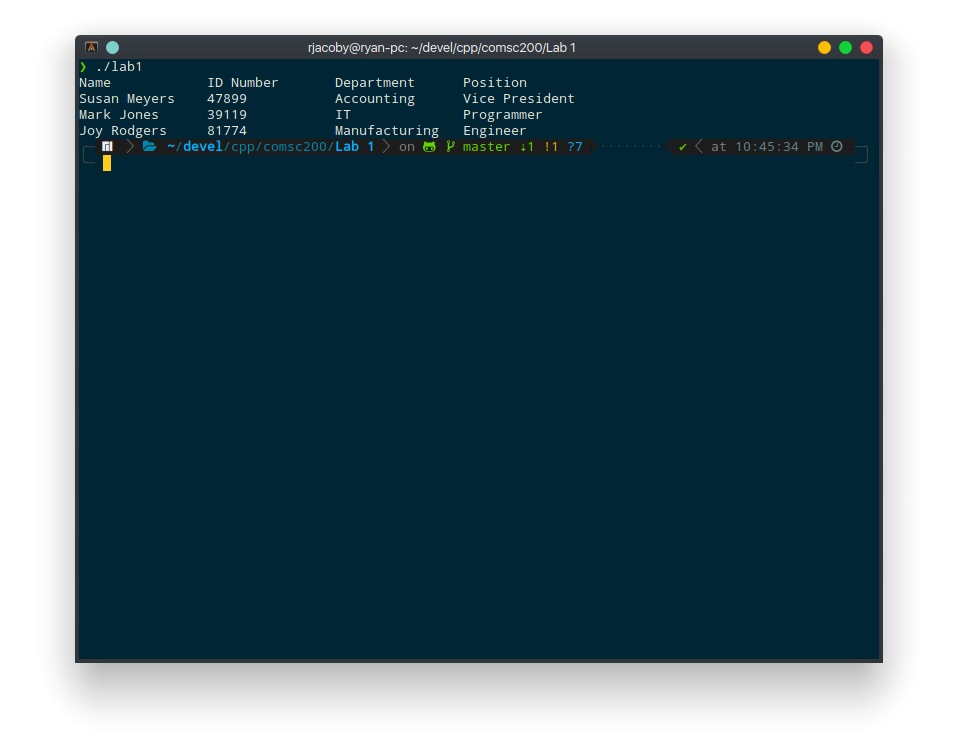
\includegraphics[scale=0.5]{employee_run.png} 

\section{Car}

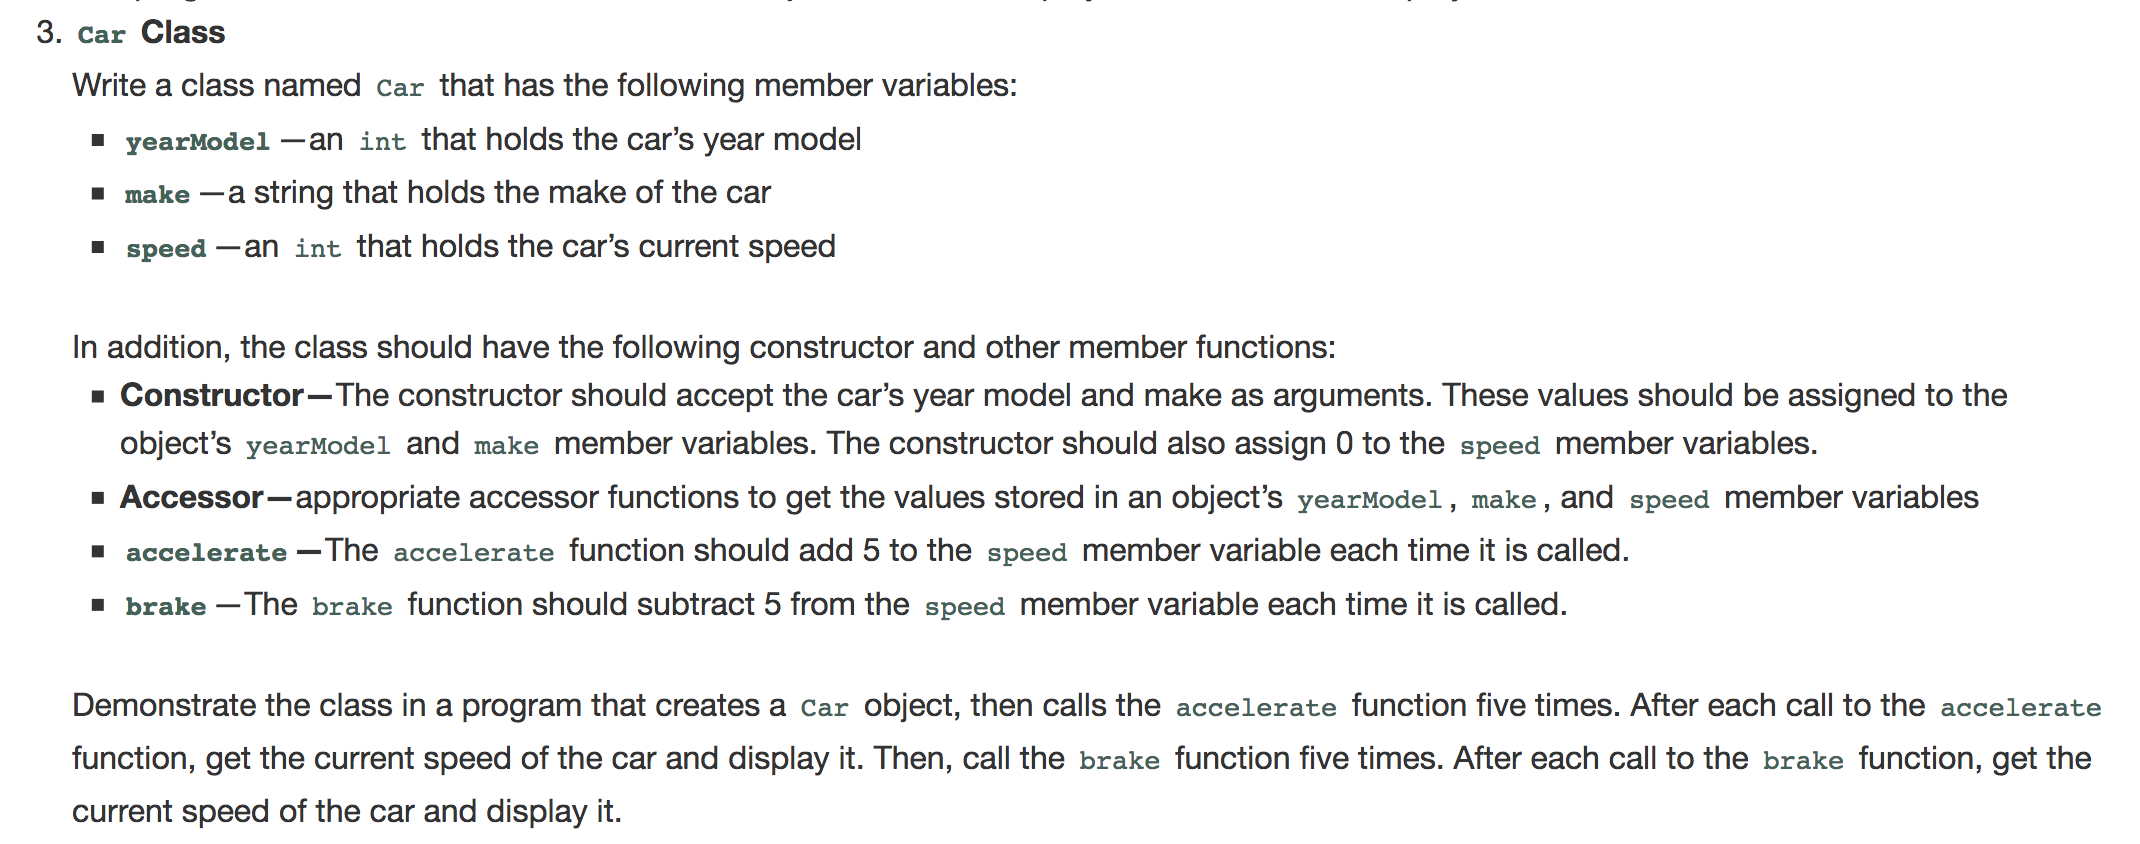
\includegraphics[scale=0.35]{car.png} 

\begin{lstlisting}[language=C++, caption=main.cpp]
// Ryan Jacoby

#include<iostream>

#include"Car.h"

using namespace std;

int main() {
    Car c = Car(2020, "Virtual Car");

    cout << "New car created\n Year: " << c.getYearModel() << "\nModel: " << c.getMake() << '\n';

    for(int i = 0; i < 5; i++) {
        cout << "Car current speed: " << c.getSpeed() << '\n';
        c.accelerate();
    }

    cout << "Car current speed: " << c.getSpeed() << '\n';

    for(int i = 0; i < 5; i++) {
        cout << "Car current speed: " << c.getSpeed() << '\n';
        c.brake();
    }

    return 0;
}
\end{lstlisting}

\begin{lstlisting}[language=C++, caption=Car.h]
// Ryan Jacoby

#ifndef Car_h
#define Car_h

using namespace std;

class Car {
private:
    int yearModel;
    string make;
    int speed;
public:
    Car(int yearModel, string make);

    int getYearModel() { return this->yearModel; }
    string getMake() { return this->make; }
    int getSpeed() { return this->speed; }

    void accelerate();
    void brake();
};

#endif
\end{lstlisting}

\begin{lstlisting}[language=C++, caption=CarImp.cpp]
// Ryan Jacoby

#include<string>

#include"Car.h"

using namespace std;

Car::Car(int yearModel, string make) {
    this->yearModel = yearModel;
    this->make = make;
    this->speed = 0;
}

void Car::accelerate() {
    speed += 5;
}

void Car::brake() {
    speed -= 5;
}
\end{lstlisting}

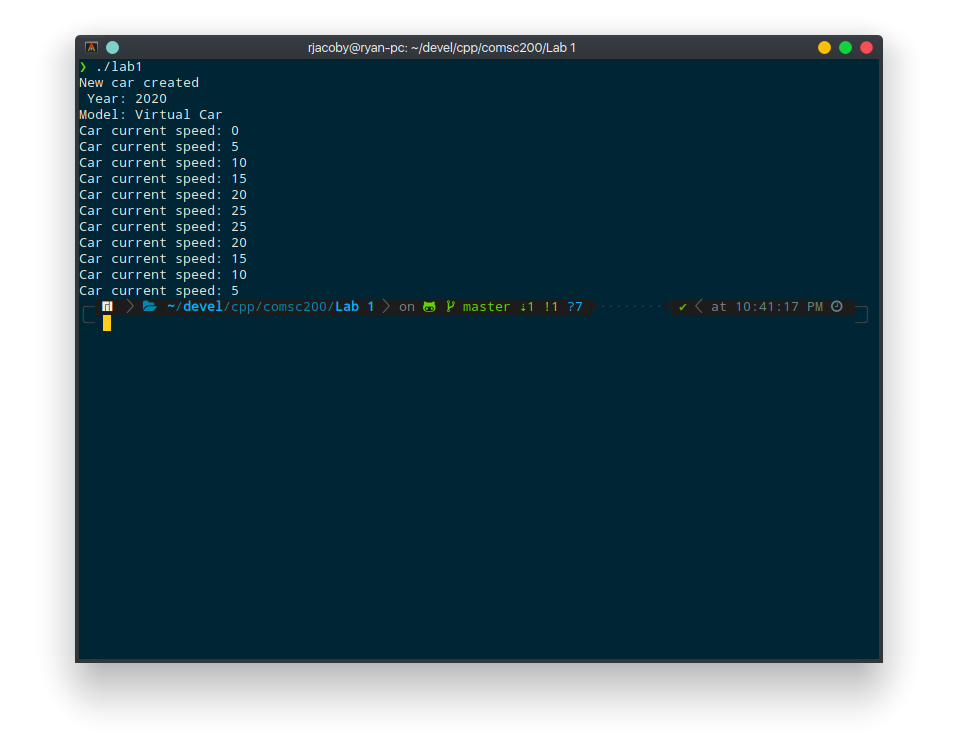
\includegraphics[scale=0.5]{car_run.png} 

\section{Circle}

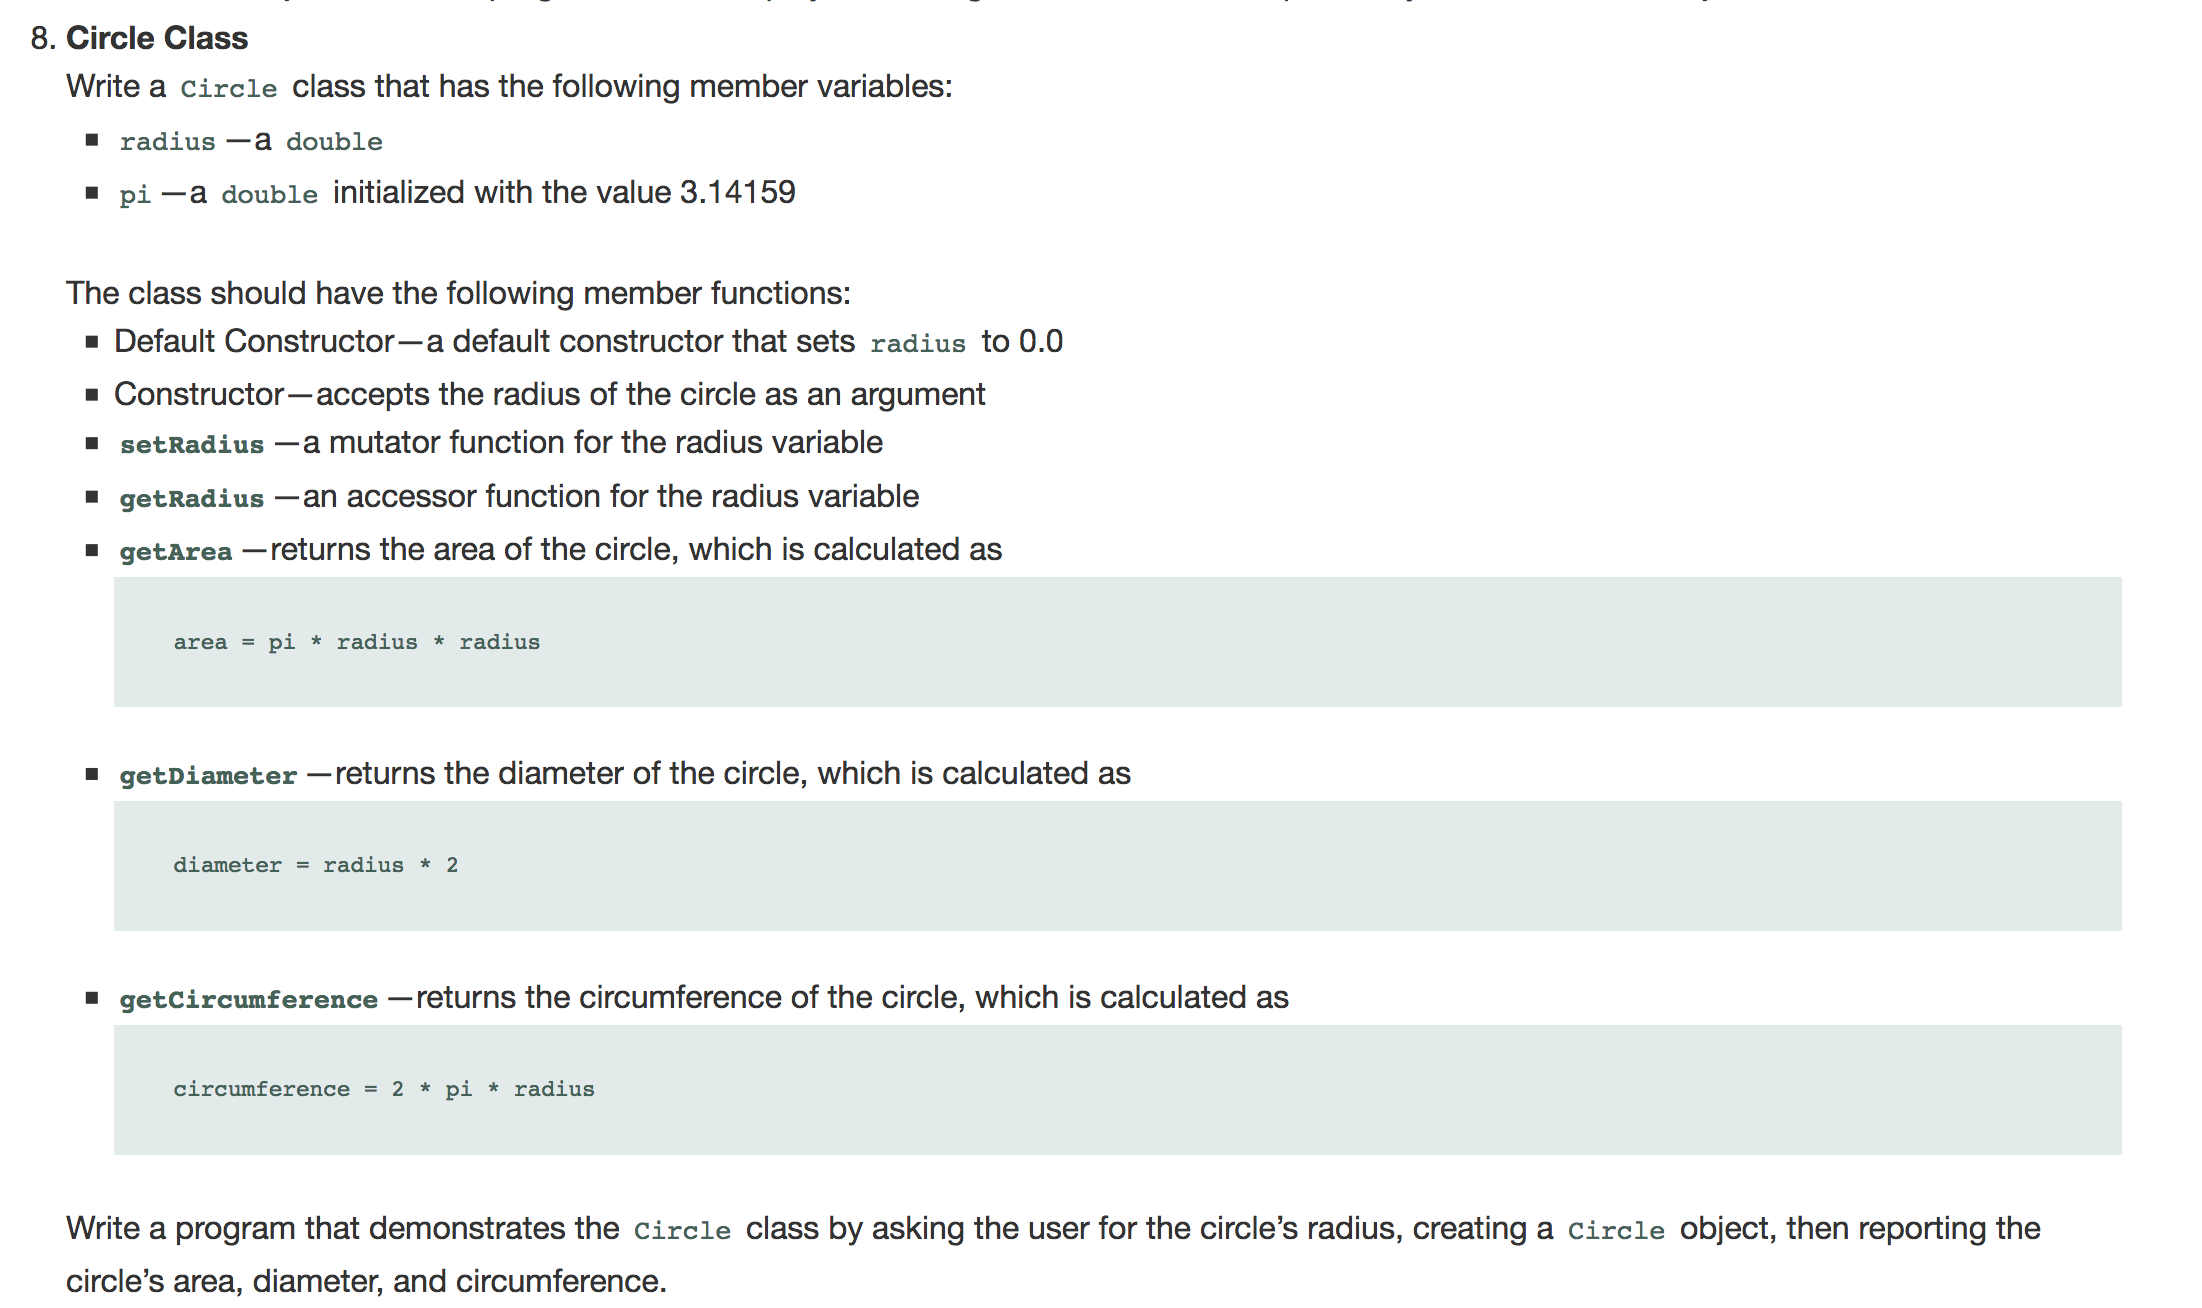
\includegraphics[scale=0.35]{circle.png} 

\begin{lstlisting}[language=C++, caption=main.cpp]
// Ryan Jacoby

#include<iostream>

#include"Circle.h"

using namespace std;

int main() {
    double rad;
    Circle c = Circle();

    cout << "What size circle do you want: ";
    cin >> rad;
    
    c.setRadius(rad);

    cout << "That circle has an area of " << c.getArea() << ", a diameter of " << c.getDiameter() << ", and a circumference of " << c.getCircumference() << ".\n";

    return 0;
}
\end{lstlisting}

\begin{lstlisting}[language=C++, caption=Circle.h]
// Ryan Jacoby

#ifndef Circle_h
#define Circle_h

class Circle {
private:
    double radius;
    double pi;
public:
    Circle();
    Circle(double radius);

    void setRadius(double radius) { this->radius = radius; }
    double getRadius() { return this->radius; }
    
    double getArea();
    double getDiameter();
    double getCircumference();
};

#endif
\end{lstlisting}

\begin{lstlisting}[language=C++, caption=CircleImp.cpp]
// Ryan Jacoby

#include"Circle.h"

Circle::Circle() {
    this->radius = 0;
    this->pi = 3.14159;
}

Circle::Circle(double radius) {
    this->radius = radius;
    this->pi = 3.14159;
}

double Circle::getArea() {
    return this->pi * this->radius * this->radius;
}

double Circle::getDiameter() {
    return this->radius * 2;
}

double Circle::getCircumference() {
    return this->pi * this->radius * 2;
}
\end{lstlisting}

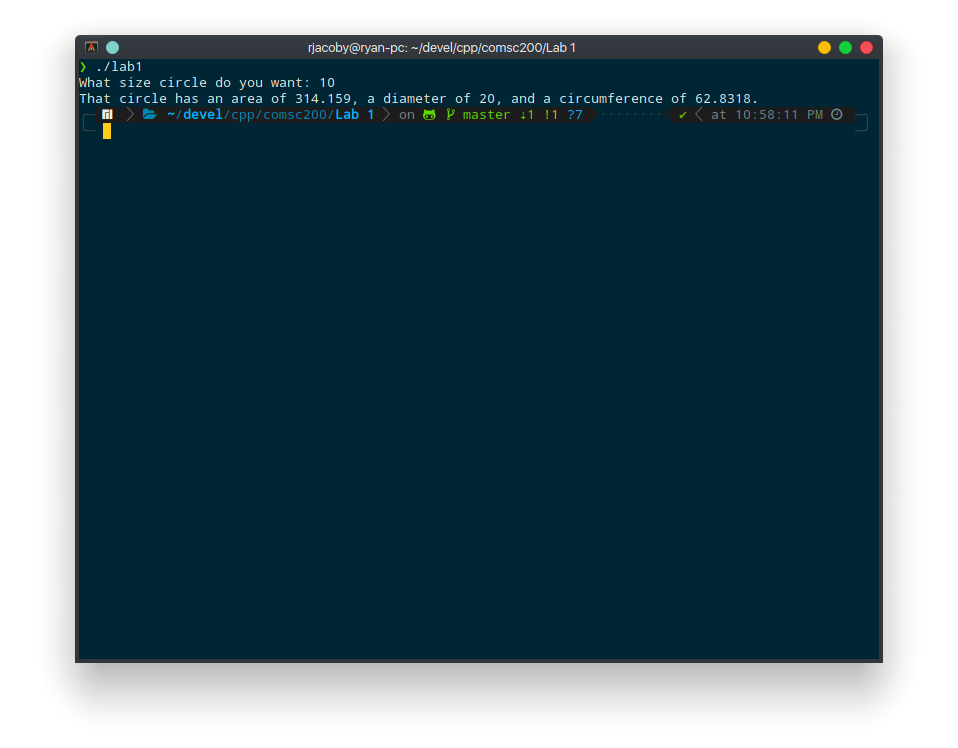
\includegraphics[scale=0.5]{circle_run.png} 

\section{Number Array}

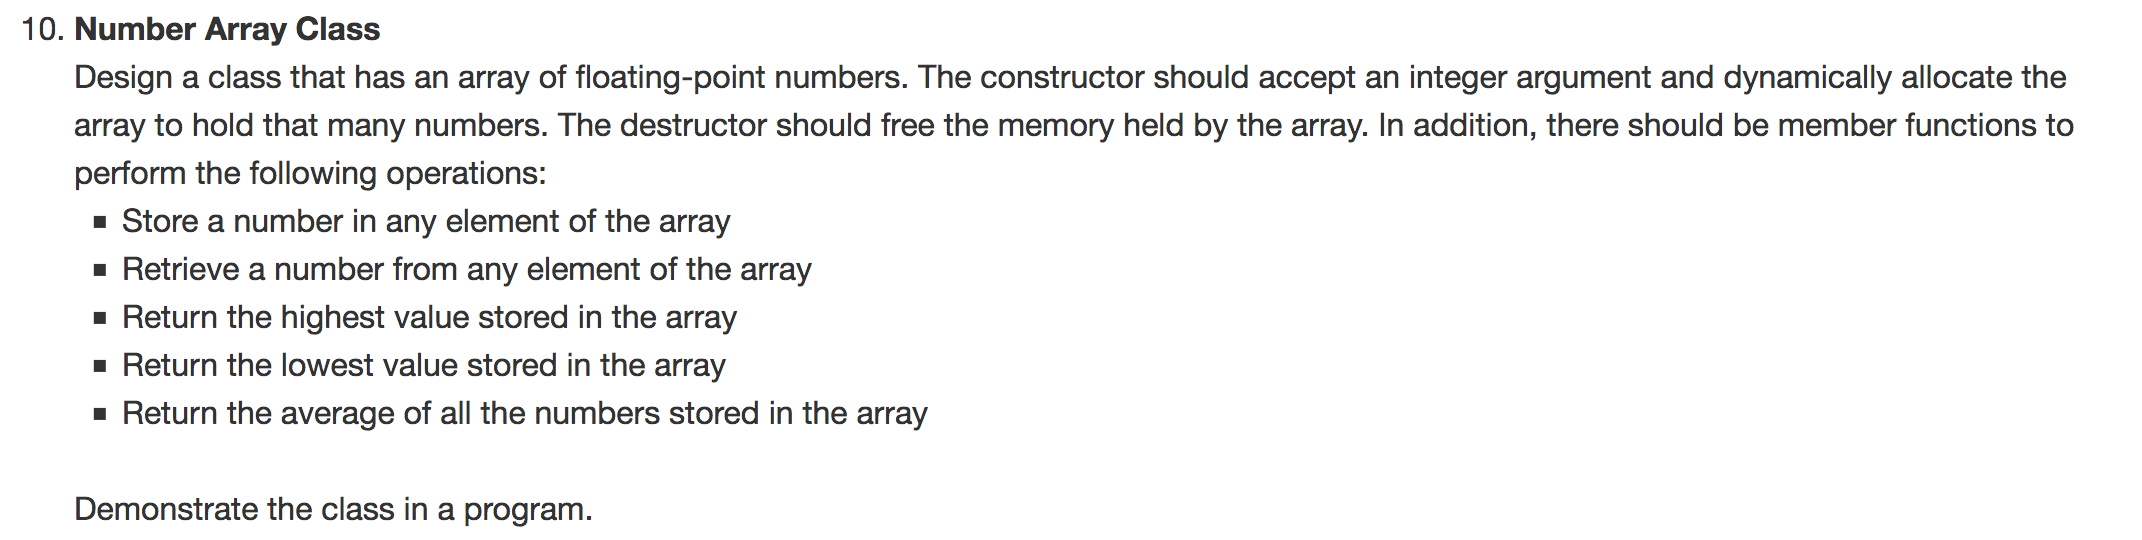
\includegraphics[scale=0.35]{numbers.png} 

\begin{lstlisting}[language=C++, caption=main.cpp]
// Ryan Jacoby

#include<iostream>

#include"NumArray.h"

using namespace std;

int main() {
    NumArray n = NumArray(5);

    n.storeNumber(1, 1.5);
    n.storeNumber(0, 2);
    n.storeNumber(2, 2.5);
    n.storeNumber(4, 3);
    n.storeNumber(3, 3.5);

    cout << "1st number: " << n.getNumber(0) << '\n';
    cout << "Highest number: " << n.highestNum() << '\n';
    cout << "Lowest number: " << n.lowestNum() << '\n';
    cout << "Average of numbers: " << n.average() << '\n';

    return 0;
}
\end{lstlisting}

\begin{lstlisting}[language=C++, caption=NumArray.h]
// Ryan Jacoby

#ifndef NumArray_h
#define NumArray_h

class NumArray {
private:
    double * nums;
    int elements;
public:
    NumArray(int elements);

    ~NumArray();

    void storeNumber(int pos, double num);
    double getNumber(int pos);
    double highestNum();
    double lowestNum();
    double average();
};

#endif
\end{lstlisting}

\begin{lstlisting}[language=C++, caption=NumArrayImp.cpp]
// Ryan Jacoby

#include"NumArray.h"

NumArray::NumArray(int elements) {
    this->elements = elements;
    this->nums = new double[elements];
}

NumArray::~NumArray() {
    delete[] this->nums;
}

void NumArray::storeNumber(int pos, double num){
    this->nums[pos] = num;
}

double NumArray::getNumber(int pos) {
    return this->nums[pos];
}

double NumArray::highestNum() {
    double highest = this->nums[0];

    for(int i = 0; i < elements; i++) {
        if(this->nums[i] > highest) highest = this->nums[i];
    }

    return highest;
}

double NumArray::lowestNum() {
    double lowest = this->nums[0];
    
    for(int i = 0; i < elements; i++) {
        if(this->nums[i] < lowest) lowest = this->nums[i];
    }

    return lowest;
}

double NumArray::average() {
    double sum = 0;

    for(int i = 0; i < elements; i++) 
        sum += this->nums[i];

    return sum / elements;
}
\end{lstlisting}

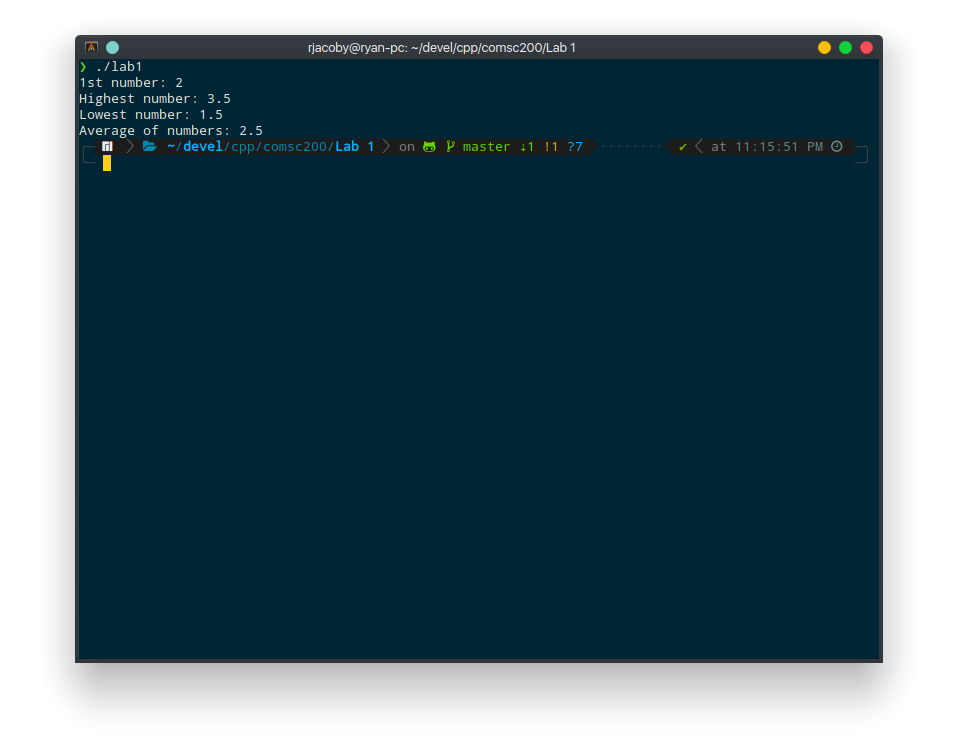
\includegraphics[scale=0.5]{numbers_run.png} 

\section{Coin}

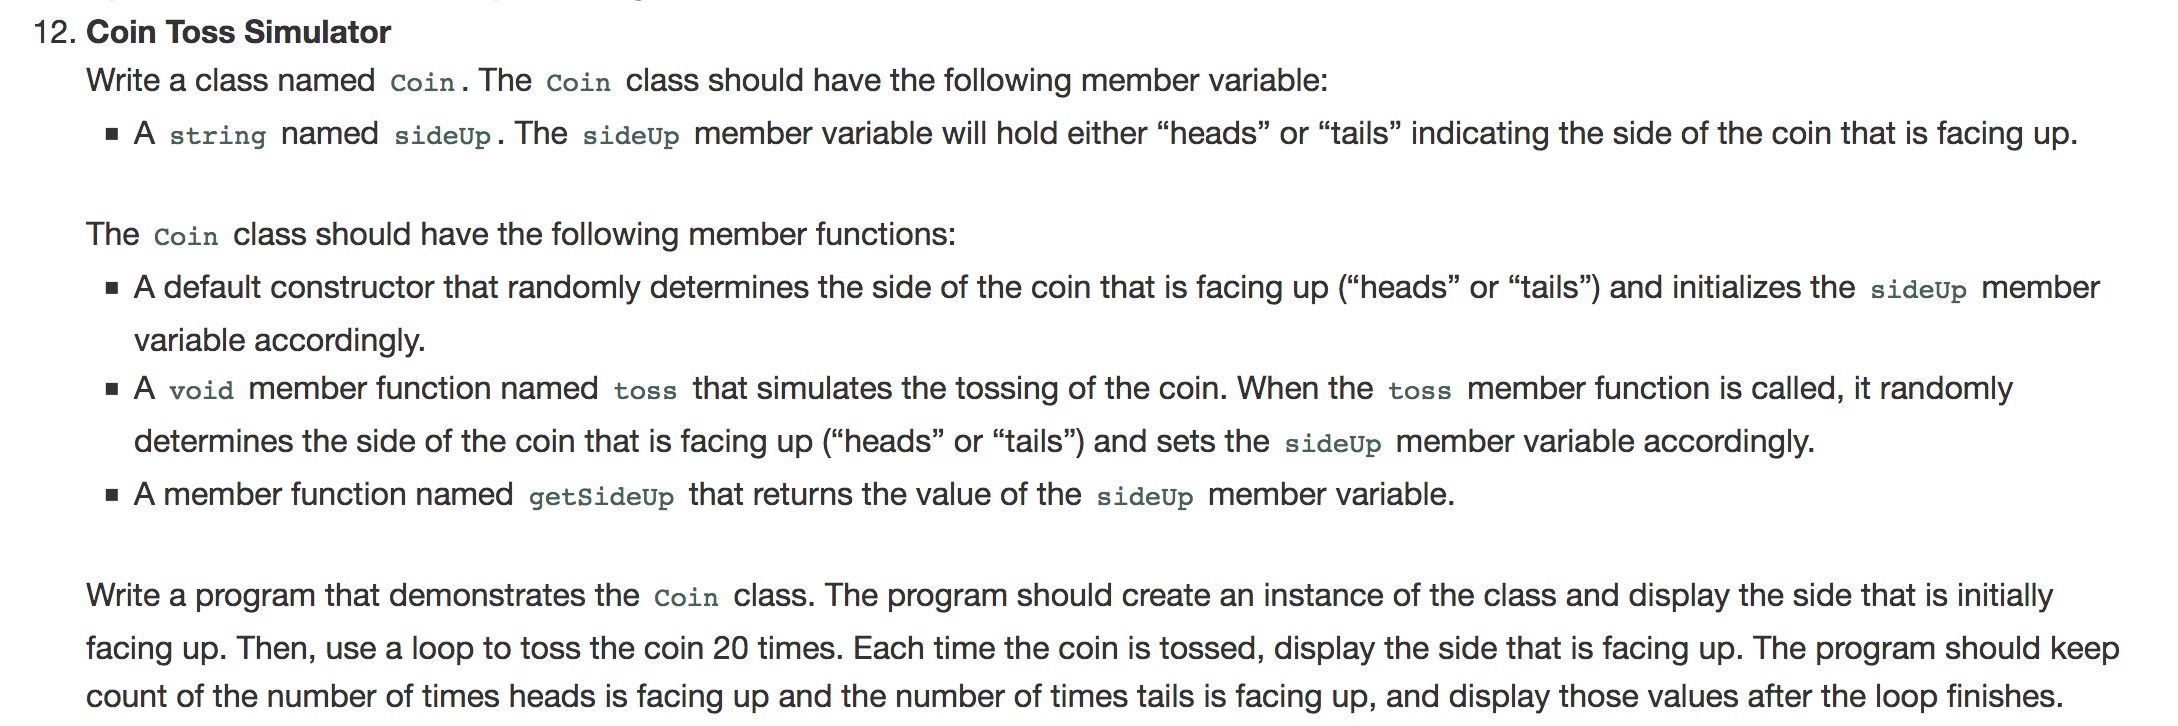
\includegraphics[scale=0.35]{coin.png} 

\begin{lstlisting}[language=C++, caption=main.cpp]
// Ryan Jacoby

#include<iostream>

#include"Coin.h"

using namespace std;

int main() {
    Coin c = Coin();

    for(int i = 0; i < 20; i++) {
        cout << "Coin was " << c.getSideUp() << '\n';
        c.toss();
    }

    return 0;
}
\end{lstlisting}

\begin{lstlisting}[language=C++, caption=Coin.h]
// Ryan Jacoby

#ifndef Coin_h
#define Coin_h

using namespace std;

class Coin {
private:
    string sideUp;
public:
    Coin();

    void toss();
    string getSideUp();
};

#endif
\end{lstlisting}

\begin{lstlisting}[language=C++, caption=CoinImp.cpp]
// Ryan Jacoby

#include<string>

#include<stdlib.h>
#include<time.h>

#include"Coin.h"

using namespace std;

Coin::Coin() {
    srand(time(NULL));

    if(rand() % 2 == 0) this->sideUp = "heads";
    else this->sideUp = "tails";
}

void Coin::toss() {
    if(rand() % 2 == 0) this->sideUp = "heads";
    else this->sideUp = "tails";
}

string Coin::getSideUp() {
    return this->sideUp;
}
\end{lstlisting}

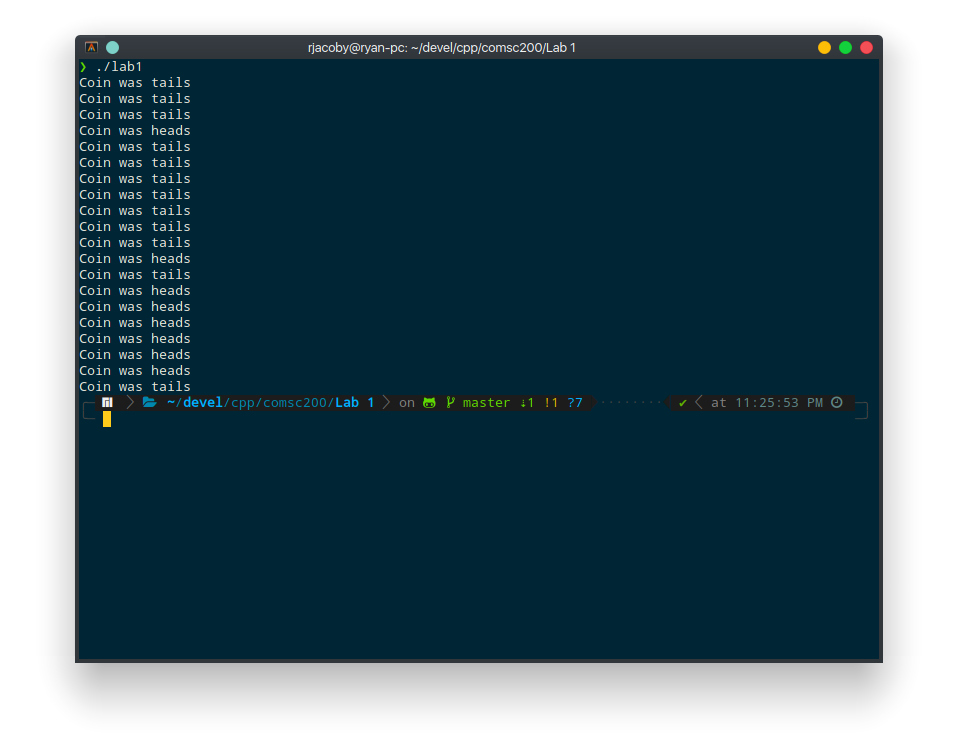
\includegraphics[scale=0.5]{coin_run.png} 

\end{document}
